\documentclass[10pt,a4paper]{article}
\usepackage[utf8]{inputenc}
\usepackage{amsmath}
\usepackage{amsfonts}
\usepackage{amssymb}
\usepackage{mathtools}
\usepackage{tensor}
\author{Andreas Forster}
\numberwithin{equation}{section}
\renewcommand{\vec}[1]{\ensuremath{\mathbf{#1}}}
\newcommand{\vecs}[1]{\ensuremath{\boldsymbol{#1}}}
\newcommand{\mat}[1]{\ensuremath{\mathbf{#1}}}
\renewcommand{\deg}{\ensuremath{^\circ}}
\newcommand{\norm}[1]{\ensuremath{\left|\left|#1\right|\right|}}
\newcommand{\Exp}{\mathrm{Exp}}
\newcommand{\Log}{\mathrm{Log}}
\newcommand{\stplus}{\boxplus}
\newcommand{\pluseq}{\mathrel{+}=}
\newcommand{\minuseq}{\mathrel{-}=}

\renewcommand{\arraystretch}{1.5}
%\setcounter{secnumdepth}{0}

\begin{document}
\section{Definitions}
$\Phi$ bijective mapping from minimal coordinates to tangent space.\\
Perturbation around estimate $\bar{\vec{x}}$: $\delta\vec{x} = \vec{x}\stplus\bar{\vec{x}}^{-1}$
\begin{align*}
\delta\vec{x} &= \exp(\Phi(\delta\vecs{\chi})) \eqqcolon \Exp(\vecs{\chi})\\
\delta\vecs{\chi} &= \Phi^{-1}(\log(\delta\vec{x})) \eqqcolon \Log(\delta\vec{x})
\end{align*}
Parameter Block $\leftrightarrow$ State\\
Residual Block $\leftrightarrow$ Error term, measurement...

\section{The Marginalization Error Term}
The steps to marginalize out a certain state in the code is:
\begin{enumerate}
\item Add all related residual blocks to the marginalization error term.
\item Marginalize the parameter blocks.
\item Update error computation before next optimization.
\end{enumerate}

\subsection{Adding a residual block}
Firstly all the states / parameter blocks related to this residual block are found. If this state is not yet related to the marginalization error term, the Hessian $\mat{H}$ and the right hand side vector $\vec{b}$ is resized accordingly. The values of $\mat{H}$ and $\vec{b}$  are shuffled around to make sure the sparsity pattern remains the same. Landmark states are added at the end and the others are added in between the 'dense' part and the 'sparse/landmark' part. See Figure \ref{fig:sparsity_pattern} for a visualisation. The new areas are set to zero.
\begin{figure}[h]
\centering
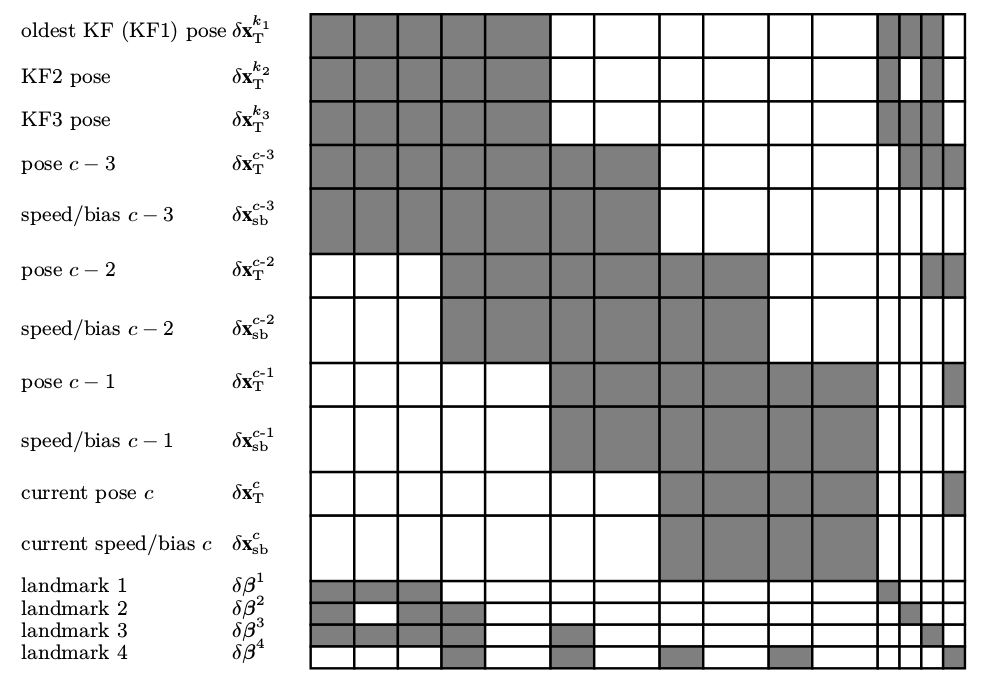
\includegraphics[width=\textwidth]{sparsity_pattern.png}
\caption{Sparsity pattern of Hessian. \cite{LeuteneggerPHD}}
\label{fig:sparsity_pattern}
\end{figure}
The current estimate of the parameters are saved as linearization point.\\
The residual $\vec{r}$ and the (minimal) jacobians $J_{i}$ of the error term with respect to the parameters $i$ are calculated. Some magic is done with the Jacobians if the loss function is not quadratic.\\
$\mat{H}$ and $\vec{b}$ are updated at the right location:
\begin{align}
\mat{H}.\texttt{block}(idx(i), idx(i), dim(i), dim(i)) &\pluseq J_i^TJ_i && \forall i\\
\mat{H}.\texttt{block}(idx(i), idx(j), dim(i), dim(j)) &\pluseq J_i^TJ_j && \forall j < i\\
\mat{H}.\texttt{block}(idx(j), idx(i), dim(j), dim(i)) &\pluseq J_j^TJ_i && \forall j < i\\
\vec{b}.\texttt{segment}(idx(i), dim(i)) &\minuseq J_i^T \vec{r} && \forall i
\end{align}

\subsection{Marginalization}
We want to marginalize out a few parameters.
First, the diagonal of the whole Hessian $\mat{H}$ is damped:
\begin{align}
p_i &= \sqrt{\mat{H}_{ii}}\\
\mat{H} &\leftarrow \mathrm{diag}(\vec{p})^{-1} \mat{H} \mathrm{diag}(\vec{p})^{-1}\\
\vec{b} &\leftarrow \mathrm{diag}(\vec{p})^{-1} \vec{b}
\end{align}

The Hessian $\mat{H}$ is split into 3 parts. $\mat{U}, \mat{V}$ and $\mat{W}$. $\mat{U}$ is part of the Hessian that is kept, $\mat{V}$ is the part related to the soon to be marginalized states and $\mat{W}$ is the part that is related to both things. 
The rhs $\vec{b}$ is split into 'kept' parts $\vec{b}_a$ and 'to be marginalized' part $\vec{b}_b$. The preconditioner is also split into $\vec{p}_a$ and $\vec{p}_b$.\\
Now the Schur operation begins. For this the pseudo inverse of $\mat{V}$ is calculated $\mat{V}^{+}$
\begin{align}
\mat{H} &= \mat{U} - \mat{W}\mat{V}^{+}\mat{W}^T\\
\vec{b} &= \vec{b}_a - \mat{W} \mat{V}^+\vec{b}_b
\end{align}

And now the Hessian $\mat{H}$ and rhs $\vec{b}$ are unscaled again.
\begin{align}
\mat{H} &\leftarrow \mathrm{diag}(\vec{p}_a) \mat{H} \mathrm{diag}(\vec{p}_a)\\
\vec{b} &\leftarrow \mathrm{diag}(\vec{p}_a) \vec{b}
\end{align}

\subsection{Update error computation}
It is important that $\mat{H}$ stays positive semidefinit. Due to numeric noise this might not be the case. Therefore the eigenvalue decomposition (of the damped Hessian) $\mat{V}\mat{S}\mat{V}^T$ is calculated and all eigenvalues below a threshold are set to zero. 
The threshold is $t = \varepsilon \cdot \mat{H}.\texttt{cols()} \cdot \max_i\lambda_i$.\\
Now certain values are calculated that are used in the error calculation:
The Jacobian is 'extracted' from the decomposition.
\begin{equation}
\mat{J} = \left(\mathrm{diag}(\vec{p})V\sqrt{S}\right)^T
\end{equation}
As well as the constant error $\vec{e}_0$:
\begin{align}
(\mat{J}^T)^{-1} &= \sqrt{S^{-1}}V^T\mathrm{diag}(\vec{p})^{-1}\\
\vec{e}_0 &= -(\mat{J}^T)^{-1}\vec{b}
\end{align}

\subsection{Error calculation}
We can approximate the right hand side as:
\begin{equation}
\vec{b} \approx \vec{b}_0 + \frac{\partial\vec{b}}{\partial\Delta\vecs{\chi}} = \vec{b}_0 - \mat{H}\Delta\chi
\end{equation}
Or equivalently
\begin{equation}
\vec{e} \approx \vec{e}_0 + \mat{J} \Delta \vecs{\chi}
\end{equation}
Since 
\begin{align}
\vec{b} &= -\mat{J}^T\vec{e}\\
&\approx -\mat{J}^T \left(\vec{e}_0 + \left.\frac{\partial \vec{e}(\vec{x})}{\partial \delta\vecs{\chi}}\right|_{\vec{x}_0} \delta\vecs{\chi}\right)\\
&\approx -\mat{J}^T \left(\vec{e}_0 +  \mat{J}\delta\vecs{\chi}\right)\\
&\approx \underbrace{-\mat{J}^T\vec{e}_0}_{\vec{b}_0} - \mat{H}\delta\vecs{\chi}
\end{align}
$\Delta\vecs{\chi}$ represents the state updates that occur after marginalization. 
\begin{equation}
\Delta\vecs{\chi} = \Log(\bar{\vec{x}}\stplus\vec{x}_0^{-1}) =  \Log(\bar{\vec{x}}\boxminus\vec{x}_0)
\end{equation}
The error is:
\begin{equation}
\vec{e} = \vec{e}_0 + J \Delta\vecs{\chi}
\end{equation}

\nocite{*}
\bibliographystyle{IEEEtran}
\bibliography{refs}
\end{document}